% Compile with:
%   pdflatex 0xchou00_detection_tool.tex
%   bibtex 0xchou00_detection_tool
%   pdflatex 0xchou00_detection_tool.tex
%   pdflatex 0xchou00_detection_tool.tex
\documentclass[11pt,a4paper]{article}

\usepackage[a4paper,margin=1in]{geometry}
\usepackage[T1]{fontenc}
\usepackage[utf8]{inputenc}
\usepackage{lmodern}
\usepackage{hyperref}
\usepackage{booktabs}
\usepackage{longtable}
\usepackage{enumitem}
\usepackage{amsmath}
\usepackage{tikz}
\usetikzlibrary{positioning}
\usepackage[numbers]{natbib}

\hypersetup{
  colorlinks=true,
  linkcolor=black,
  citecolor=black,
  urlcolor=blue,
  pdftitle={0xchou00 Detection Tool},
  pdfauthor={0xchou00}
}

\title{0xchou00 Detection Tool:\\Architecture, Detection Flow, Enrichment, and Correlation}
\author{Technical documentation for the public codebase}
\date{April 17, 2026}

\begin{document}
\maketitle

\begin{abstract}
0xchou00 is intentionally not presented as a full SIEM. It is a lightweight detection tool designed for single-node operation, direct inspection, and low-friction deployment. This document explains the codebase as it exists publicly: local and API-based ingestion, normalization, IP enrichment, event-level detection, alert correlation, SQLite persistence, tamper-evident integrity, and an operator dashboard. It also explains the design boundaries that distinguish a detection tool from a large-scale SIEM deployment.
\end{abstract}

\section{Detection Tool vs. SIEM}

A SIEM usually addresses large-scale aggregation, indexing, retention, search, and cross-source analytics across many systems. NIST log-management guidance emphasizes broad collection, storage, review, and analysis processes across an organization's infrastructure \citep{nist80092}. Products such as Splunk, Elastic-based stacks, and Wazuh typically add distributed storage, scaling controls, richer search, and fleet-wide collection workflows.

0xchou00 solves a narrower problem:

\begin{itemize}[leftmargin=1.5em]
  \item collect security-relevant logs on one node;
  \item normalize them into one event model;
  \item enrich source IPs with local or cached context;
  \item apply explainable detector logic;
  \item correlate short multi-step attack patterns;
  \item preserve the result in a tamper-evident local store.
\end{itemize}

That is why the repository is described as a \textbf{security detection tool}. The choice is technical, not cosmetic.

\section{Architecture}

\begin{center}
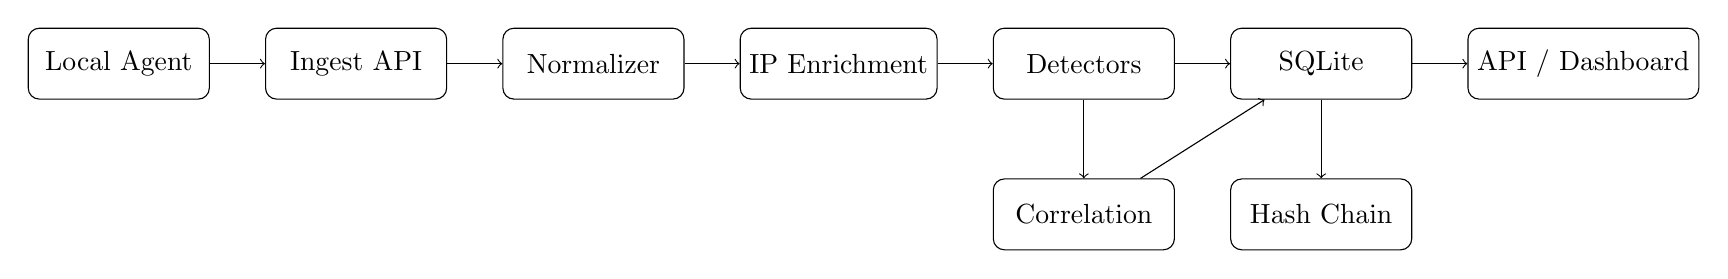
\begin{tikzpicture}[
  node distance=1cm and 0.7cm,
  box/.style={draw, rounded corners, align=center, minimum width=2.3cm, minimum height=0.9cm}
]
\node[box] (agent) {Local Agent};
\node[box, right=of agent] (apiingest) {Ingest API};
\node[box, right=of apiingest] (normalize) {Normalizer};
\node[box, right=of normalize] (enrich) {IP Enrichment};
\node[box, right=of enrich] (detect) {Detectors};
\node[box, below=of detect] (correlate) {Correlation};
\node[box, right=of detect] (store) {SQLite};
\node[box, below=of store] (chain) {Hash Chain};
\node[box, right=of store] (ui) {API / Dashboard};

\draw[->] (agent) -- (apiingest);
\draw[->] (apiingest) -- (normalize);
\draw[->] (normalize) -- (enrich);
\draw[->] (enrich) -- (detect);
\draw[->] (detect) -- (store);
\draw[->] (detect) -- (correlate);
\draw[->] (correlate) -- (store);
\draw[->] (store) -- (chain);
\draw[->] (store) -- (ui);
\end{tikzpicture}
\end{center}

This pipeline is linear on purpose. Each stage has a narrow responsibility, which keeps the code inspectable and keeps failures localized.

\section{Log Processing Pipeline}

\subsection{Ingestion}

The tool accepts log lines in two ways:

\begin{itemize}[leftmargin=1.5em]
  \item \texttt{POST /ingest} for direct API submission;
  \item a local Python agent that tails \texttt{/var/log/auth.log} and \texttt{/var/log/nginx/access.log}.
\end{itemize}

The agent uses offset and inode tracking so it can resume after restarts and recover from common log-rotation behavior. This is closer to a local collector than a demonstration script.

\subsection{Normalization}

Supported public parsers:

\begin{itemize}[leftmargin=1.5em]
  \item SSH authentication failures and successes from \texttt{sshd};
  \item Apache or Nginx combined-style web access logs.
\end{itemize}

The result is a single \texttt{LogEvent} schema with stable fields such as source type, event type, source IP, HTTP metadata, and severity. This keeps the detector layer source-aware only where necessary.

\section{Enrichment Strategy}

\subsection{Local-first Context}

The enrichment layer runs immediately after normalization. It can add:

\begin{itemize}[leftmargin=1.5em]
  \item \texttt{country};
  \item \texttt{is\_malicious};
  \item \texttt{reputation\_score};
  \item \texttt{enrichment\_source}.
\end{itemize}

The order is intentional:

\begin{enumerate}[leftmargin=1.5em]
  \item static blacklist;
  \item local GeoIP database;
  \item cached threat-intelligence data;
  \item asynchronous AbuseIPDB refresh when configured.
\end{enumerate}

\subsection{Why the External Lookup Is Asynchronous}

The detection path should not pause because a remote reputation API is slow. Therefore, first-seen IPs are enriched with whatever local context is available immediately, and optional external reputation data is fetched in the background and cached for later events. This trades first-event completeness for stable ingestion latency.

\section{Detection Logic}

\subsection{SSH Brute Force}

The brute-force detector counts failed SSH authentications per source IP inside a 60-second sliding window:

\begin{equation}
\texttt{failures}_{ip,60s} \geq 5
\end{equation}

If the source IP is already flagged as malicious or reaches three times the threshold, the alert is raised to \texttt{critical}. This reflects the role of repeated authentication failures in brute-force activity \citep{mitreT1110}.

\subsection{Suspicious Web IP Behavior}

The web detector covers three high-signal cases:

\begin{itemize}[leftmargin=1.5em]
  \item excessive request rate;
  \item excessive error ratio;
  \item access to sensitive paths such as \texttt{/.env} or \texttt{/.git/config}.
\end{itemize}

These checks are aligned with common reconnaissance and forced-browsing patterns described by OWASP and ATT\&CK scanning guidance \citep{owaspForcedBrowsing,mitreT1595Wordlist}.

\subsection{YAML Rules}

YAML rules allow field equality, substring matches, regular expressions, and grouped thresholds without editing Python. This keeps detection development simple for narrow environments.

\subsection{Frequency Anomaly}

The anomaly detector builds a short baseline from recent fixed windows and alerts when the current event count exceeds:

\begin{equation}
\max(12,\ 3 \times \mu)
\end{equation}

where $\mu$ is the average of the previous baseline windows. This is simple threshold-based anomaly detection, not a machine-learning subsystem.

\section{Correlation Logic}

Correlation is applied after detector alerts exist. It does not work on raw events; it works on recent alerts. Rules in \texttt{rules/correlation\_rules.yml} specify:

\begin{itemize}[leftmargin=1.5em]
  \item a set of required detector alerts;
  \item a time window;
  \item whether the source IP must match;
  \item output title, description, and severity.
\end{itemize}

The public examples include:

\begin{itemize}[leftmargin=1.5em]
  \item SSH brute force combined with suspicious web probing from the same source;
  \item traffic anomaly combined with sensitive path access.
\end{itemize}

Correlated alerts are stored in the same alert table as detector alerts. This keeps the API and dashboard simple because there is no separate retrieval path.

\section{Integrity}

Each stored event and alert is sealed into a chain entry:

\begin{equation}
H_n = \mathrm{SHA256}(type_n \parallel id_n \parallel payload_n \parallel H_{n-1} \parallel t_n)
\end{equation}

The hash primitive follows the Secure Hash Standard \citep{fips1804}. The higher-level design is consistent with the secure-audit-log pattern described by Schneier and Kelsey \citep{schneier1999}. The tool verifies both chain continuity and current payload hashes against stored entities. This gives tamper evidence, not distributed consensus.

\section{Security Practices}

\begin{itemize}[leftmargin=1.5em]
  \item API access uses role-ranked keys.
  \item Detector and correlation logic are data-driven where practical.
  \item Optional external threat intelligence is cached and bounded by timeout.
  \item The local agent tracks offsets to avoid replaying entire files after restart.
  \item Integrity verification is exposed through a dedicated endpoint.
\end{itemize}

\section{Alternatives and Tradeoffs}

\subsection{ELK Stack}

Elastic-based logging stacks provide scalable indexing, distributed search, and large-volume querying. They are stronger for broad telemetry retention and search, but heavier to operate than a single SQLite-backed node.

\subsection{Wazuh}

Wazuh brings host agents, rule content, and central security analytics. It is broader in host coverage, but it also introduces a larger deployment and management surface.

\subsection{Splunk}

Splunk is mature for enterprise log management and search, but it is designed for environments that need higher ingestion scale, search depth, and administrative control than this tool targets.

\subsection{Why FastAPI and SQLite Here}

FastAPI keeps the HTTP layer compact and explicit. SQLite keeps the storage path inspectable and easy to move. Those choices fit the actual scope of the codebase:

\begin{itemize}[leftmargin=1.5em]
  \item one host;
  \item one operator or small lab;
  \item one local database;
  \item direct code inspection over opaque infrastructure.
\end{itemize}

\section{Limitations}

\begin{itemize}[leftmargin=1.5em]
  \item only SSH and web access logs are normalized publicly;
  \item the dashboard is polling-based;
  \item SQLite is not intended for multi-node ingestion at scale;
  \item first-seen IPs may only have local context until the asynchronous cache refresh completes;
  \item the integrity chain cannot prevent destructive deletion by a privileged local user.
\end{itemize}

\section{Conclusion}

0xchou00 is most useful when treated honestly: a lightweight detection tool with real ingestion, enrichment, detection, correlation, and integrity features on a single node. Its main strength is that the entire path from raw line to correlated alert remains readable, debuggable, and easy to operate without external infrastructure.

\bibliographystyle{plainnat}
\bibliography{0xchou00_detection_tool_references}

\end{document}
